\chapter{球員製作過程}
\renewcommand{\baselinestretch}{10.0} %設定行距
\pagenumbering{arabic} %設定頁號阿拉伯數字
\setcounter{page}{2}  %設定頁數
\fontsize{14pt}{2.5pt}\sectionef
\section{車體改良-運行}
  原本的車體為球形 BubbleRob,雖然造型簡單,卻會有容易翻車的問題。因此改為磚塊型,在前後添加兩顆輪子保持平衡。也將前進原理改為四輪驅動,使轉彎更為順暢合理。\\[1pt]
\begin{figure}[hbt!]
\begin{center}
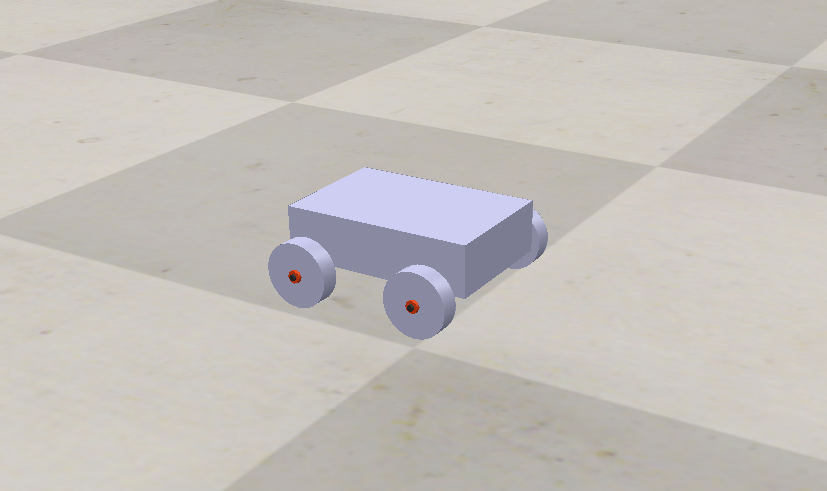
\includegraphics[height=5cm]{36}
\caption{\Large 磚塊型車體}\label{fig.36}
\end{center}
\end{figure} 
\section{車體改良-擊球}
  球員前端添加凸出的手部,球員本體在 CoppeliaSim 中用導入的開啟方式會產生抖動,因此改為加入物件 skin 並將本體隱藏。\\
\begin{figure}[hbt!]
\begin{center}
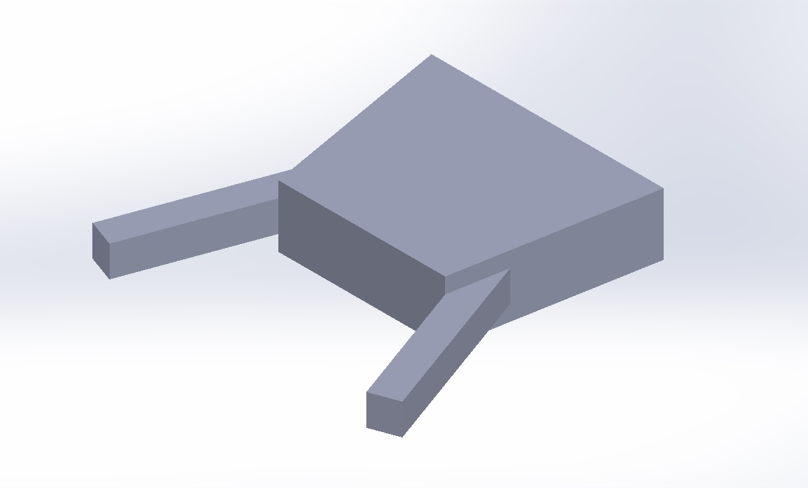
\includegraphics[height=4cm]{37}
\caption{\Large 球員 skin}\label{fig.37}
\end{center}
\end{figure} 
\newpage
\section{車體改良-背號}
  由於兩隊各有四名球員,場上總共八名球員,為了能更清楚觀看及辨別球員,除了透過顏色區分隊伍,也需要讓每個球員添加背號。第一版的背號是直立式置於球員上方,實際遊玩時發現會有影響重心的問題。\\
\begin{figure}[hbt!]
\begin{center}
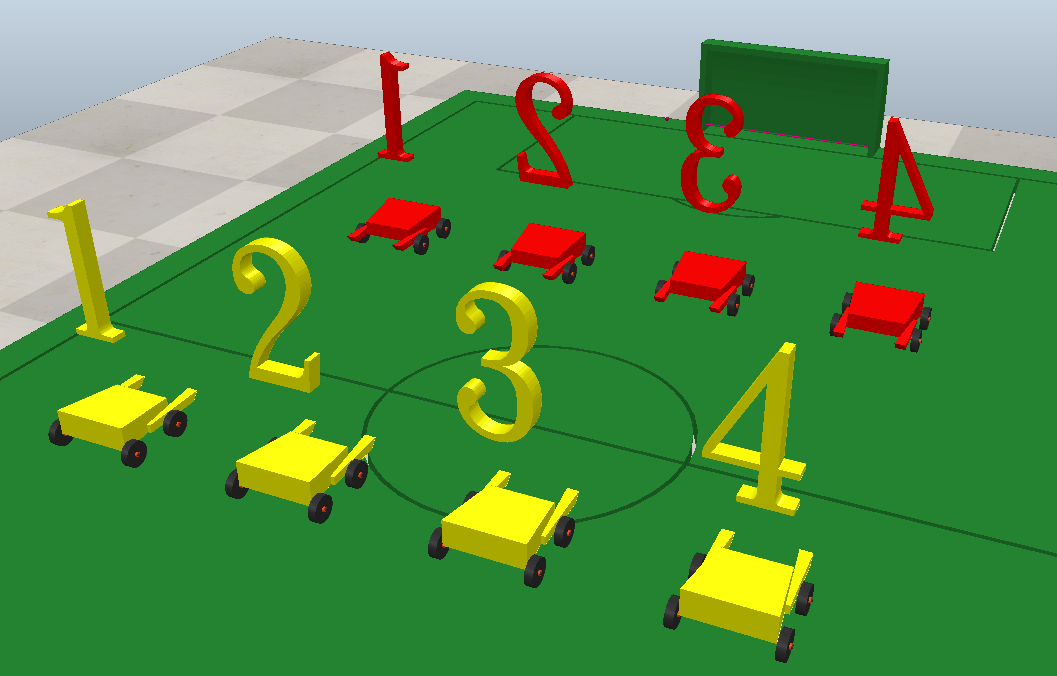
\includegraphics[height=6cm]{38}
\caption{\Large 第一版球員背號}\label{fig.38}
\end{center}
\end{figure}


於是第二版做了調整,參考實際賽車都將編號繪於車身,我們將背號改為平貼於車頂,解決了影響重心的問題。\\
\begin{figure}[hbt!]
\begin{center}
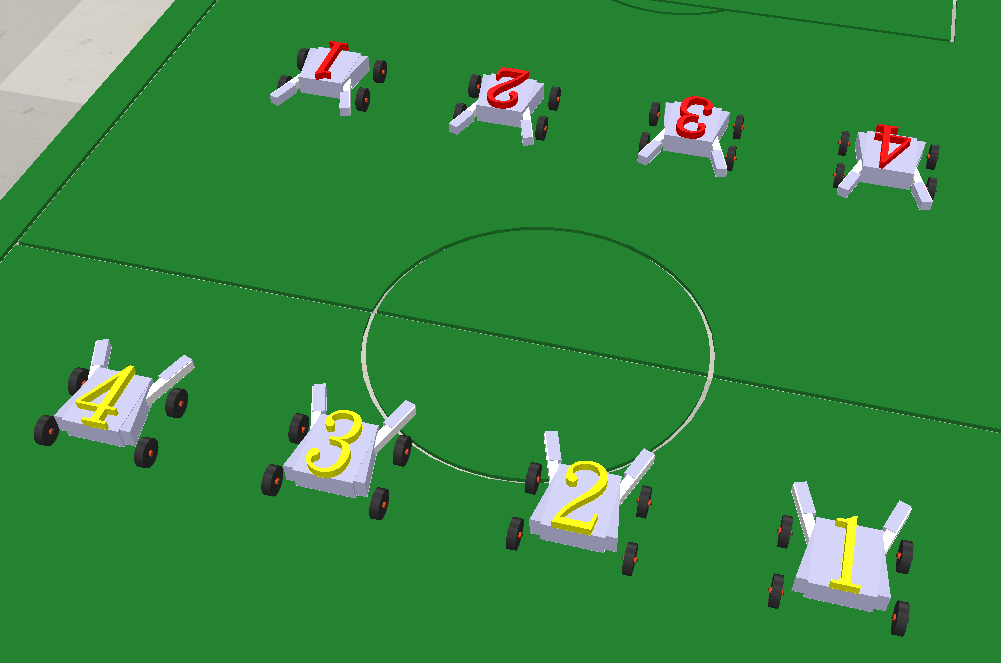
\includegraphics[height=6cm]{39}
\caption{\Large 第二版球員背號}\label{fig.39}
\end{center}
\end{figure}

\renewcommand{\baselinestretch}{1} %設定行距